\section{Рабочий проект}
\subsection{Описание компонентов и классов программы}
\subsubsection{Описание классов сервиса аутентификации}
\paragraph{Описание класса AuthController}

Описание полей и методов класса AuthController представлено в таблицах \ref{classAuthFields:table} и \ref{classAuthMethods:table} соответственно.

\renewcommand{\arraystretch}{0.8} % уменьшение расстояний до сетки таблицы
\begin{xltabular}{\textwidth}{|X|p{2.5cm}|>{\setlength{\baselineskip}{0.7\baselineskip}}p{4.83cm}|>{\setlength{\baselineskip}{0.7\baselineskip}}p{4.85cm}|}
	\caption{Описание полей класса AuthController}\label{classAuthFields:table}
	\hline \centrow \setlength{\baselineskip}{0.7\baselineskip} Название поля & \centrow \setlength{\baselineskip}{0.7\baselineskip} Область видимости & \centrow Тип данных & \centrow Описание \\
	\hline \centrow 1 & \centrow 2 & \centrow 3 & \centrow 4\\ \hline
	\endfirsthead
	\continuecaption{Продолжение таблицы \ref{classAuthFields:table}}
	\hline \centrow 1 & \centrow 2 & \centrow 3 & \centrow 4\\ \hline
	\finishhead
	dbContext & private & ChatDbContext & Контекст базы данных приложения\\
	\hline jwtService & private & JwtService & Сервис, отвечающий за работу с jwt-токенами \\
\end{xltabular}
\renewcommand{\arraystretch}{1.0}

\begin{xltabular}{\textwidth}{|X|p{2.5cm}|>{\setlength{\baselineskip}{0.7\baselineskip}}p{4.83cm}|}
	\caption{Описание методов класса AuthController}\label{classAuthMethods:table}
	\hline \centrow Название поля & \centrow Область видимости & \centrow Описание \\ \hline \centrow 1 & \centrow 2 & \centrow 3\\
	\hline 
	\endfirsthead
	\continuecaption{Продолжение таблицы \ref{classAuthMethods:table}}
	\hline \centrow 1 & \centrow 2 & \centrow 3 \\ \hline
	\hline \centrow Название поля & \centrow Область видимости & \centrow Описание \\ \hline
	\endhead
	SignUp & public & Действие контроллера, отвечающее за регистрацию пользователей \\ \hline
	SignIn & public & Действие контроллера, отвечающее за авторизацию пользователей \\ \hline
\end{xltabular}

\renewcommand{\arraystretch}{1.0}

\paragraph{Описание класса TokensController}

Описание полей и методов класса TokensController представлено в таблицах \ref{classTokensFields:table} и \ref{classTokensMethods:table} соответственно.

\renewcommand{\arraystretch}{0.8} % уменьшение расстояний до сетки таблицы
\begin{xltabular}{\textwidth}{|X|p{2.5cm}|>{\setlength{\baselineskip}{0.7\baselineskip}}p{4.83cm}|>{\setlength{\baselineskip}{0.7\baselineskip}}p{4.85cm}|}
	\caption{Описание полей класса AuthController}\label{classTokensFields:table}
	\hline \centrow \setlength{\baselineskip}{0.7\baselineskip} Название поля & \centrow \setlength{\baselineskip}{0.7\baselineskip} Область видимости & \centrow Тип данных & \centrow Описание \\
	\hline \centrow 1 & \centrow 2 & \centrow 3 & \centrow 4\\ \hline
	\endfirsthead
	\continuecaption{Продолжение таблицы \ref{classTokensFields:table}}
	\hline \centrow 1 & \centrow 2 & \centrow 3 & \centrow 4\\ \hline
	\finishhead
	dbContext & private & ChatDbContext & Контекст базы данных приложения\\
	\hline jwtService & private & JwtService & Сервис, отвечающий за работу с jwt-токенами \\
\end{xltabular}
\renewcommand{\arraystretch}{1.0}

\begin{xltabular}{\textwidth}{|X|p{2.5cm}|>{\setlength{\baselineskip}{0.7\baselineskip}}p{4.83cm}|}
	\caption{Описание методов класса AuthController}\label{classTokensMethods:table}
	\hline \centrow Название поля & \centrow Область видимости & \centrow Описание \\ \hline \centrow 1 & \centrow 2 & \centrow 3\\
	\hline 
	\endfirsthead
	\continuecaption{Продолжение таблицы \ref{classTokensMethods:table}}
	\hline \centrow 1 & \centrow 2 & \centrow 3 \\ \hline
	\hline \centrow Название поля & \centrow Область видимости & \centrow Описание \\ \hline
	\endhead
	GetChatToken & public & Действие контроллера, отвечающее за выдачу токенов конкретного чата \\ \hline
	RefreshAccessToken & public & Действие контроллера, отвечающее за обновление токена доступа \\ \hline
	RefreshChatToken & public & Действие контроллера, отвечающее за обновление токенов чатов \\ \hline
\end{xltabular}

\renewcommand{\arraystretch}{1.0}

\paragraph{Описание класса JwtService}

Описание полей и методов класса JwtService представлено в таблицах \ref{classJwtFields:table} и \ref{classJwtMethods:table} соответственно.

\renewcommand{\arraystretch}{0.8} % уменьшение расстояний до сетки таблицы
\begin{xltabular}{\textwidth}{|X|p{2.5cm}|>{\setlength{\baselineskip}{0.7\baselineskip}}p{4.83cm}|>{\setlength{\baselineskip}{0.7\baselineskip}}p{4.85cm}|}
	\caption{Описание полей класса JwtService}\label{classJwtFields:table}
	\hline \centrow \setlength{\baselineskip}{0.7\baselineskip} Название поля & \centrow \setlength{\baselineskip}{0.7\baselineskip} Область видимости & \centrow Тип данных & \centrow Описание \\
	\hline \centrow 1 & \centrow 2 & \centrow 3 & \centrow 4\\ \hline
	\endfirsthead
	\continuecaption{Продолжение таблицы \ref{classJwtFields:table}}
	\hline \centrow 1 & \centrow 2 & \centrow 3 & \centrow 4\\ \hline
	\finishhead
	configuration & private & IConfiguration & Данное поле обеспечивает к конфигурации приложения\\
\end{xltabular}
\renewcommand{\arraystretch}{1.0}

\begin{xltabular}{\textwidth}{|X|p{2.5cm}|>{\setlength{\baselineskip}{0.7\baselineskip}}p{4.83cm}|}
	\caption{Описание методов класса JwtService}\label{classJwtMethods:table}
	\hline \centrow Название поля & \centrow Область видимости & \centrow Описание \\ \hline \centrow 1 & \centrow 2 & \centrow 3\\
	\hline 
	\endfirsthead
	\continuecaption{Продолжение таблицы \ref{classJwtMethods:table}}
	\hline \centrow 1 & \centrow 2 & \centrow 3 \\ \hline
	\hline \centrow Название поля & \centrow Область видимости & \centrow Описание \\ \hline
	\endhead
	GetAccessToken & public & Метод, отвечающий за генерацию токенов доступа \\ \hline
	GetRefreshToken & public & Метод, отвечающий за генерацию токенов обновления \\ \hline
	GetChatToken & public & Метод, отвечающий за генерацию токенов чатов \\ \hline
\end{xltabular}

\renewcommand{\arraystretch}{1.0}

\subsubsection{Описание классов приложения}

\paragraph{Описание класса ChatController}

Описание полей и методов класса ChatController представлено в таблицах \ref{classChatFields:table} и \ref{classChatMethods:table} соответственно.

\renewcommand{\arraystretch}{0.8} % уменьшение расстояний до сетки таблицы
\begin{xltabular}{\textwidth}{|X|p{2.5cm}|>{\setlength{\baselineskip}{0.7\baselineskip}}p{4.83cm}|>{\setlength{\baselineskip}{0.7\baselineskip}}p{4.85cm}|}
	\caption{Описание полей класса ChatController}\label{classChatFields:table}
	\hline \centrow \setlength{\baselineskip}{0.7\baselineskip} Название поля & \centrow \setlength{\baselineskip}{0.7\baselineskip} Область видимости & \centrow Тип данных & \centrow Описание \\
	\hline \centrow 1 & \centrow 2 & \centrow 3 & \centrow 4\\ \hline
	\endfirsthead
	\continuecaption{Продолжение таблицы \ref{classChatFields:table}}
	\hline \centrow 1 & \centrow 2 & \centrow 3 & \centrow 4\\ \hline
	\finishhead
	dbContext & private & ChatDbContext & Контекст базы данных приложения\\
	\hline hubContext & private & IHubContext<ChatHub> & Контекст хаба чатов, для возможности рассылки обновлений пользователям чата в реальном времени \\
\end{xltabular}
\renewcommand{\arraystretch}{1.0}

\begin{xltabular}{\textwidth}{|X|p{2.5cm}|>{\setlength{\baselineskip}{0.7\baselineskip}}p{4.83cm}|}
	\caption{Описание методов класса AuthController}\label{classChatMethods:table}
	\hline \centrow Название поля & \centrow Область видимости & \centrow Описание \\ \hline \centrow 1 & \centrow 2 & \centrow 3\\
	\hline 
	\endfirsthead
	\continuecaption{Продолжение таблицы \ref{classChatMethods:table}}
	\hline \centrow 1 & \centrow 2 & \centrow 3 \\ \hline
	\hline \centrow Название метода & \centrow Область видимости & \centrow Описание \\ \hline
	\endhead
	SendMessage & public & Метод, отвечающий за отправку сообщения в чат \\ \hline
	DeleteMessage & public & Метод, отвечающий за удаление сообщения из чата \\ \hline
	GetMessages & public & Метод, возвращающий все сообщения чата \\ \hline
	GetUsers & public & Метод, возвращающий всех пользователей в чате \\ \hline
	DeleteUser & public & Метод, отвечающий за удаление пользователя из чата \\ \hline
\end{xltabular}

\renewcommand{\arraystretch}{1.0}

\paragraph{Описание класса ChatsController}

Описание полей и методов класса ChastController представлено в таблицах \ref{classChatsFields:table} и \ref{classChatsMethods:table} соответственно.

\renewcommand{\arraystretch}{0.8} % уменьшение расстояний до сетки таблицы
\begin{xltabular}{\textwidth}{|X|p{2.5cm}|>{\setlength{\baselineskip}{0.7\baselineskip}}p{4.83cm}|>{\setlength{\baselineskip}{0.7\baselineskip}}p{4.85cm}|}
	\caption{Описание полей класса ChatsController}\label{classChatsFields:table}
	\hline \centrow \setlength{\baselineskip}{0.7\baselineskip} Название поля & \centrow \setlength{\baselineskip}{0.7\baselineskip} Область видимости & \centrow Тип данных & \centrow Описание \\
	\hline \centrow 1 & \centrow 2 & \centrow 3 & \centrow 4\\ \hline
	\endfirsthead
	\continuecaption{Продолжение таблицы \ref{classChatsFields:table}}
	\hline \centrow 1 & \centrow 2 & \centrow 3 & \centrow 4\\ \hline
	\finishhead
	dbContext & private & ChatDbContext & Контекст базы данных приложения \\
\end{xltabular}
\renewcommand{\arraystretch}{1.0}

\begin{xltabular}{\textwidth}{|X|p{2.5cm}|>{\setlength{\baselineskip}{0.7\baselineskip}}p{4.83cm}|}
	\caption{Описание методов класса ChatsController}\label{classChatsMethods:table}
	\hline \centrow Название поля & \centrow Область видимости & \centrow Описание \\ \hline \centrow 1 & \centrow 2 & \centrow 3\\
	\hline 
	\endfirsthead
	\continuecaption{Продолжение таблицы \ref{classChatsMethods:table}}
	\hline \centrow 1 & \centrow 2 & \centrow 3 \\ \hline
	\hline \centrow Название метода & \centrow Область видимости & \centrow Описание \\ \hline
	\endhead
	AddNewChat & public & Метод, отвечающий за добавление нового чата \\ \hline
	DeleteChat & public & Метод, отвечающий за удаление чата \\ \hline
	UpdateChat & public & Метод, отвечающий за обновлении информации о чате \\ \hline
\end{xltabular}

\renewcommand{\arraystretch}{1.0}

\paragraph{Описание класса UserController}

Описание полей и методов класса UserController представлено в таблицах \ref{classUserFields:table} и \ref{classUserMethods:table} соответственно.

\renewcommand{\arraystretch}{0.8} % уменьшение расстояний до сетки таблицы
\begin{xltabular}{\textwidth}{|X|p{2.5cm}|>{\setlength{\baselineskip}{0.7\baselineskip}}p{4.83cm}|>{\setlength{\baselineskip}{0.7\baselineskip}}p{4.85cm}|}
	\caption{Описание полей класса UserController}\label{classUserFields:table}
	\hline \centrow \setlength{\baselineskip}{0.7\baselineskip} Название поля & \centrow \setlength{\baselineskip}{0.7\baselineskip} Область видимости & \centrow Тип данных & \centrow Описание \\
	\hline \centrow 1 & \centrow 2 & \centrow 3 & \centrow 4\\ \hline
	\endfirsthead
	\continuecaption{Продолжение таблицы \ref{classUserFields:table}}
	\hline \centrow 1 & \centrow 2 & \centrow 3 & \centrow 4\\ \hline
	\finishhead
	dbContext & private & ChatDbContext & Контекст базы данных приложения \\
\end{xltabular}
\renewcommand{\arraystretch}{1.0}

\begin{xltabular}{\textwidth}{|X|p{2.5cm}|>{\setlength{\baselineskip}{0.7\baselineskip}}p{4.83cm}|}
	\caption{Описание методов класса ChatsController}\label{classUserMethods:table}
	\hline \centrow Название поля & \centrow Область видимости & \centrow Описание \\ \hline \centrow 1 & \centrow 2 & \centrow 3\\
	\hline 
	\endfirsthead
	\continuecaption{Продолжение таблицы \ref{classUserMethods:table}}
	\hline \centrow 1 & \centrow 2 & \centrow 3 \\ \hline
	\hline \centrow Название метода & \centrow Область видимости & \centrow Описание \\ \hline
	\endhead
	GetUserChats & public & Метод, отвечающий за получение чатов, в которых состоит пользователь \\ \hline
	GetUserInvitations & public & Метод, отвечающий за получение приглашений пользователя в чаты \\ \hline
\end{xltabular}

\renewcommand{\arraystretch}{1.0}

\paragraph{Описание класса UserController}

Описание полей и методов класса UsersController представлено в таблицах \ref{classUsersFields:table} и \ref{classUsersMethods:table} соответственно.

\renewcommand{\arraystretch}{0.8} % уменьшение расстояний до сетки таблицы
\begin{xltabular}{\textwidth}{|X|p{2.5cm}|>{\setlength{\baselineskip}{0.7\baselineskip}}p{4.83cm}|>{\setlength{\baselineskip}{0.7\baselineskip}}p{4.85cm}|}
	\caption{Описание полей класса UserController}\label{classUsersFields:table}
	\hline \centrow \setlength{\baselineskip}{0.7\baselineskip} Название поля & \centrow \setlength{\baselineskip}{0.7\baselineskip} Область видимости & \centrow Тип данных & \centrow Описание \\
	\hline \centrow 1 & \centrow 2 & \centrow 3 & \centrow 4\\ \hline
	\endfirsthead
	\continuecaption{Продолжение таблицы \ref{classUsersFields:table}}
	\hline \centrow 1 & \centrow 2 & \centrow 3 & \centrow 4\\ \hline
	\finishhead
	dbContext & private & ChatDbContext & Контекст базы данных приложения \\
\end{xltabular}
\renewcommand{\arraystretch}{1.0}

\begin{xltabular}{\textwidth}{|X|p{2.5cm}|>{\setlength{\baselineskip}{0.7\baselineskip}}p{4.83cm}|}
	\caption{Описание методов класса ChatsController}\label{classUsersMethods:table}
	\hline \centrow Название поля & \centrow Область видимости & \centrow Описание \\ \hline \centrow 1 & \centrow 2 & \centrow 3\\
	\hline 
	\endfirsthead
	\continuecaption{Продолжение таблицы \ref{classUsersMethods:table}}
	\hline \centrow 1 & \centrow 2 & \centrow 3 \\ \hline
	\hline \centrow Название метода & \centrow Область видимости & \centrow Описание \\ \hline
	\finishhead
	DeleteUser & public & Метод, отвечающий за удаление пользователя \\ \hline
	UpdateUser & public & Метод, отвечающий за обновление данных пользователя \\ \hline
\end{xltabular}

\renewcommand{\arraystretch}{1.0}

\subsection{Тестирование программной системы}

\subsubsection{Системное тестирование}

Для проверки работоспособности разработанной программной системы было произведено системное тестирование приложения. На нижеприведенных рисунках представлены результаты тестирования системы.

Произведем тестирование функционала регистрации в приложении. Для этого необходимо ввести данные для регистрациии и нажать кнопку "<Зарегистрироваться">. После регистрации пользователь должен быть перенаправлен на основную страницу приложения. Результаты тестирования данного функционала представлены на рисунках \ref{signup_test1:image}-\ref{signup_test3:image}. 

\begin{figure}[H]
	\center{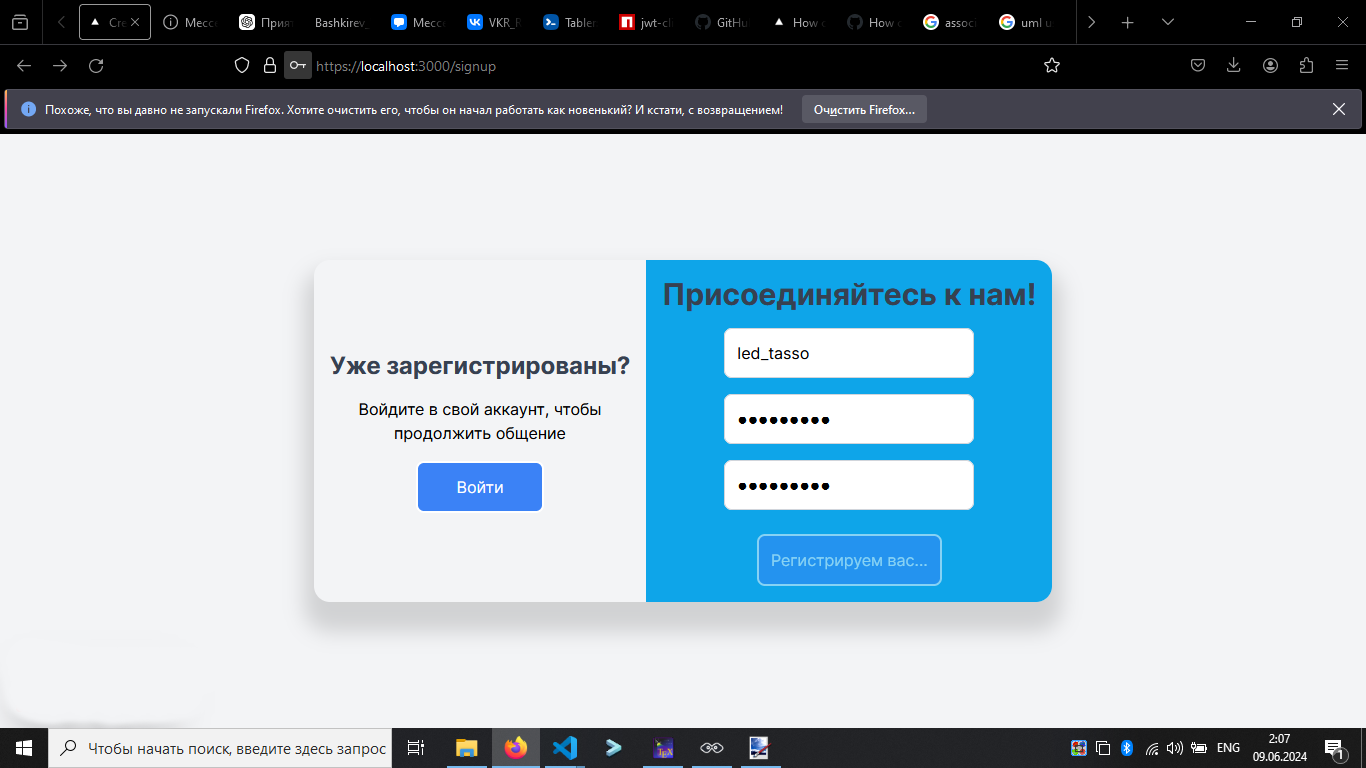
\includegraphics[width=1\linewidth]{signup_test1}}
	\caption{Процесс регистрации пользователя}
	\label{signup_test1:image}
\end{figure}

\begin{figure}[H]
	\center{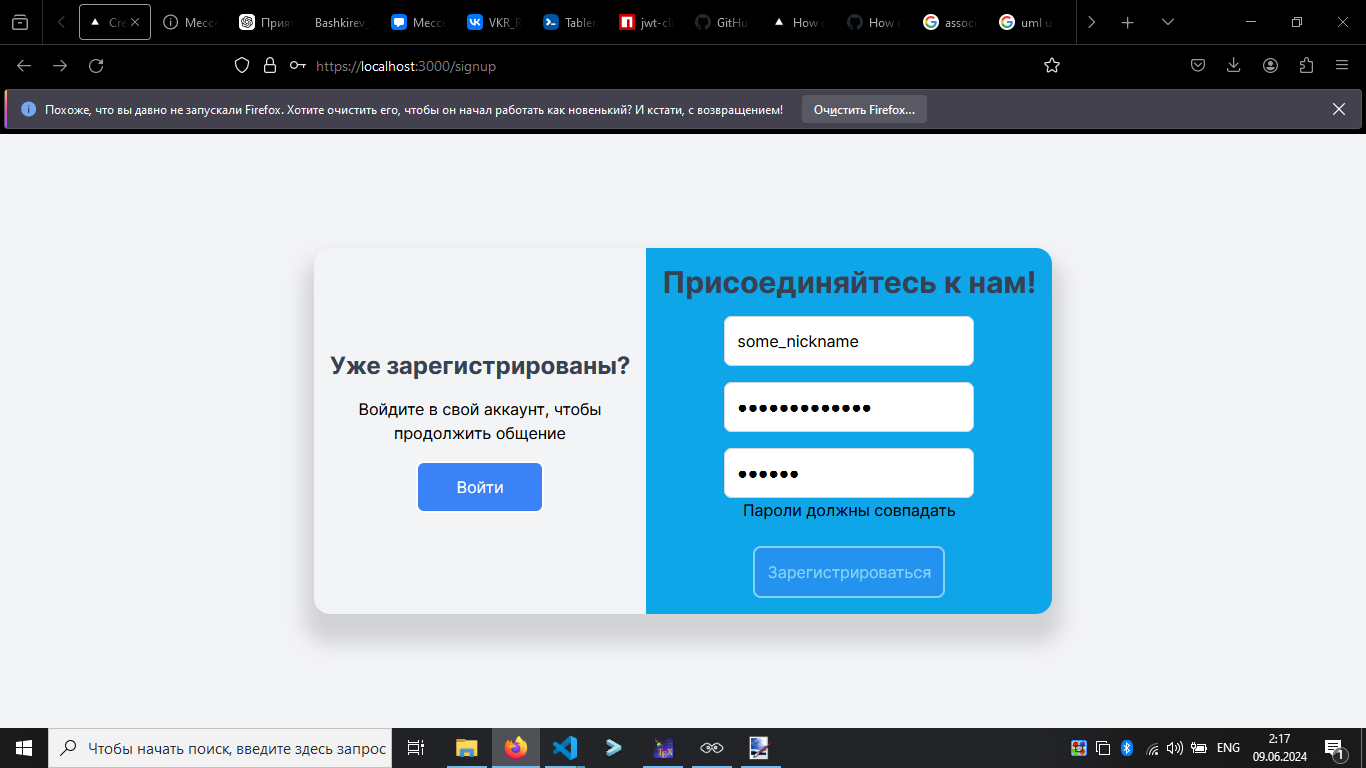
\includegraphics[width=1\linewidth]{signup_test2}}
	\caption{Попытка регистрации с неверными данными}
	\label{signup_test2:image}
\end{figure}

\begin{figure}[H]
	\center{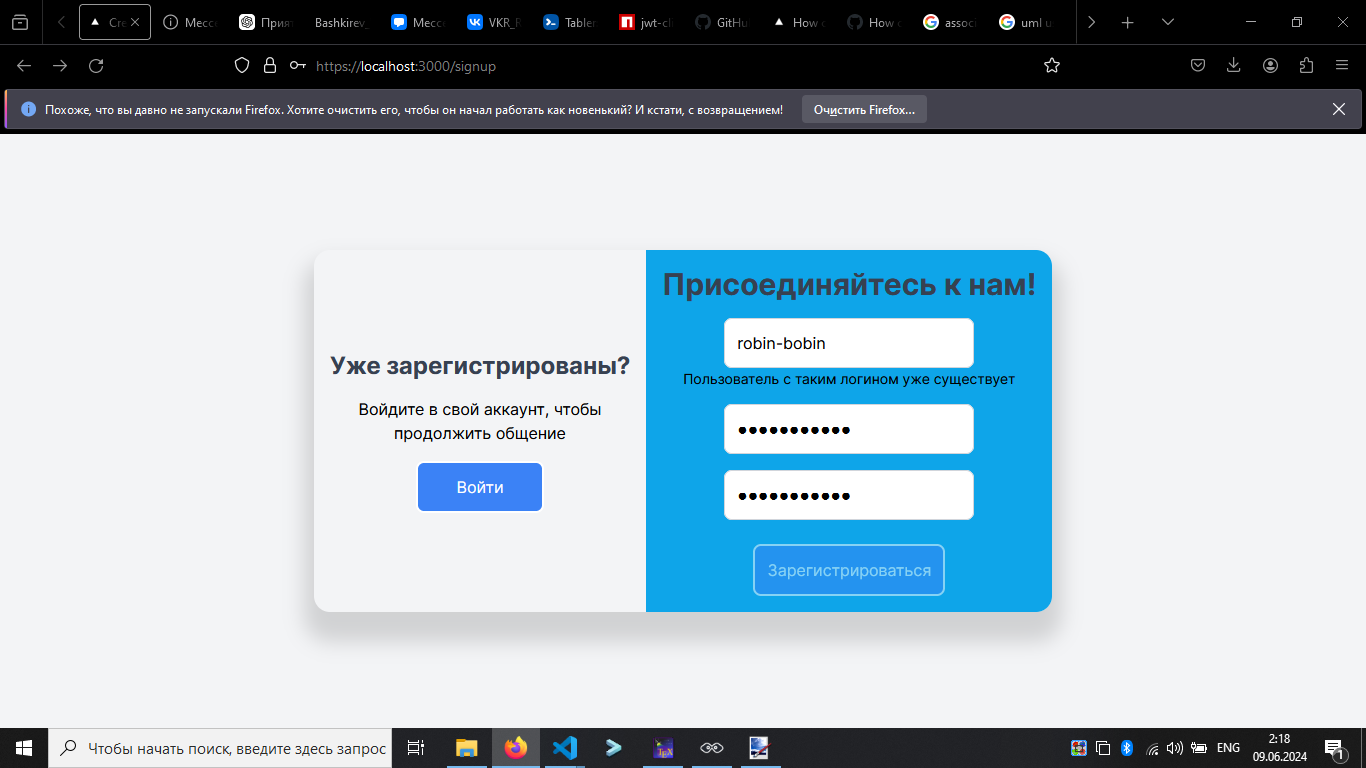
\includegraphics[width=1\linewidth]{signup_test3}}
	\caption{Попытка регистрациии с занятым логином}
	\label{signup_test3:image}
\end{figure}

После регистрации пользователь попадает на главную страницу. Результат представлен на рисунке \ref{signup_test4:image}.

\begin{figure}[H]
	\center{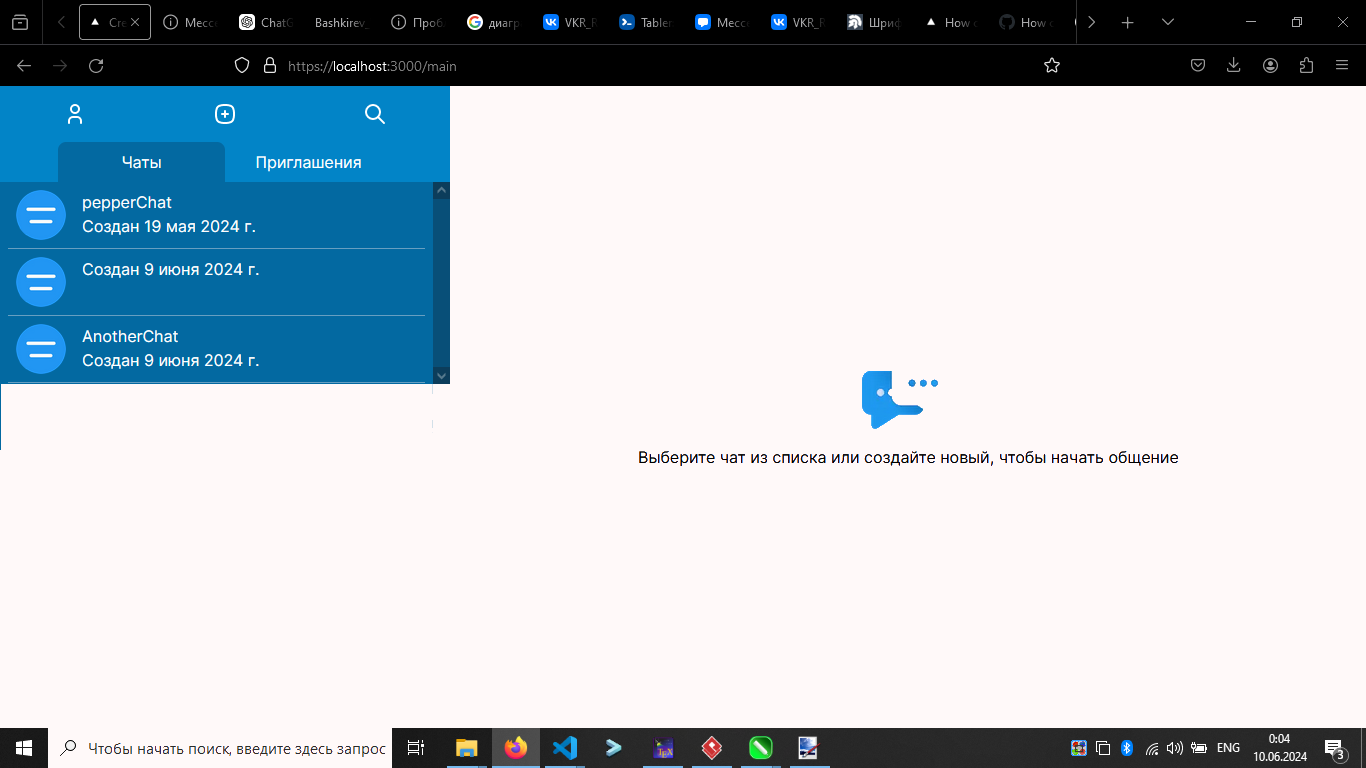
\includegraphics[width=1\linewidth]{signup_test4}}
	\caption{Переадресация на главную страницу приложения}
	\label{signup_test4:image}
\end{figure}

Приозведем тестирование функционала изменения личных данных в кабинете пользователя. Для этого попробуем изменить логин пользователя. Результаты тестирования представлены на рисунках \ref{cabinet_test1:image} и \ref{cabinet_test1:image}.


\begin{figure}[H]
	\center{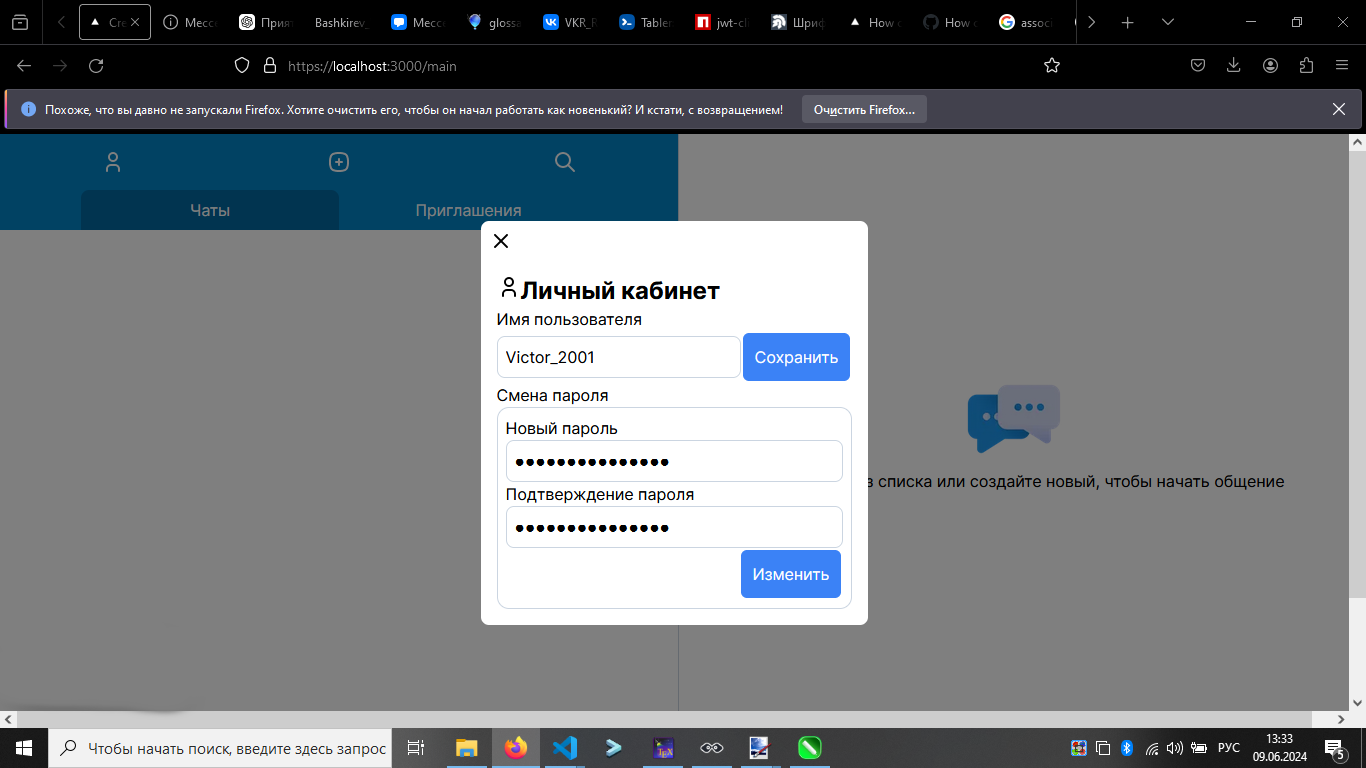
\includegraphics[width=1\linewidth]{cabinet_test1}}
	\caption{Личный кабинет пользователя с исходным логином}
	\label{cabinet_test1:image}
\end{figure}

\begin{figure}[H]
	\center{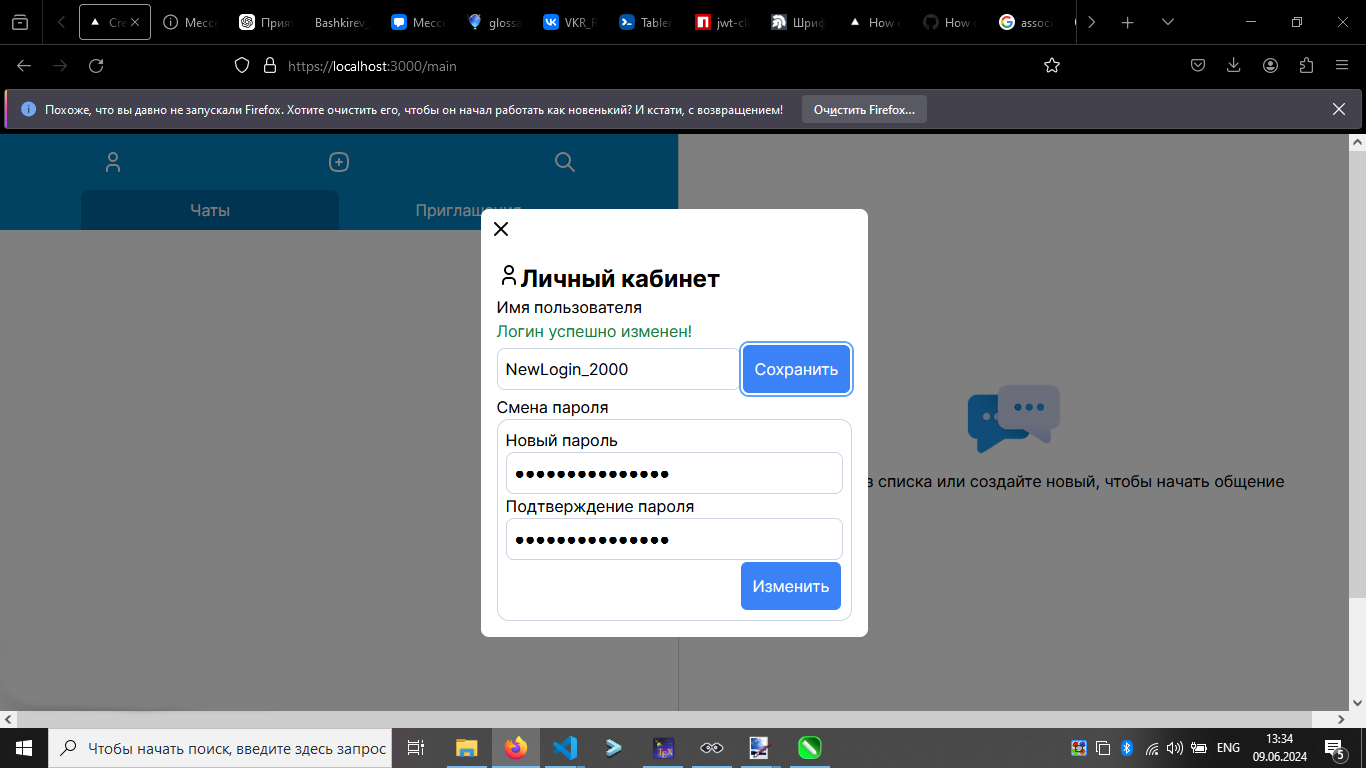
\includegraphics[width=1\linewidth]{cabinet_test2}}
	\caption{Результат изменения логина}
	\label{cabinet_test2:image}
\end{figure}

Далее протестируем функционал создания нового чата. Результаты тестов представлены на рисунках.

\begin{figure}[H]
	\center{\includegraphics[width=1\linewidth]{newChat_test1}}
	\caption{Ввод имени нового чата}
	\label{newChat_test1:image}
\end{figure}

\begin{figure}[H]
	\center{\includegraphics[width=1\linewidth]{newChat_test2}}
	\caption{Сообщение о успешном создании нового чата}
	\label{newChat_test2:image}
\end{figure}

\begin{figure}[H]
	\center{\includegraphics[width=1\linewidth]{newChat_test3}}
	\caption{Новый чат в списке чатов пользователя}
	\label{newChat_test3:image}
\end{figure}

Произведем тестирование функционала отправки сообщения. Для этого введем в поле ввода сообщения его текст и нажмем кнопку "<Отправить">. Результаты тестирования представлен на рисунках.

\begin{figure}[H]
	\center{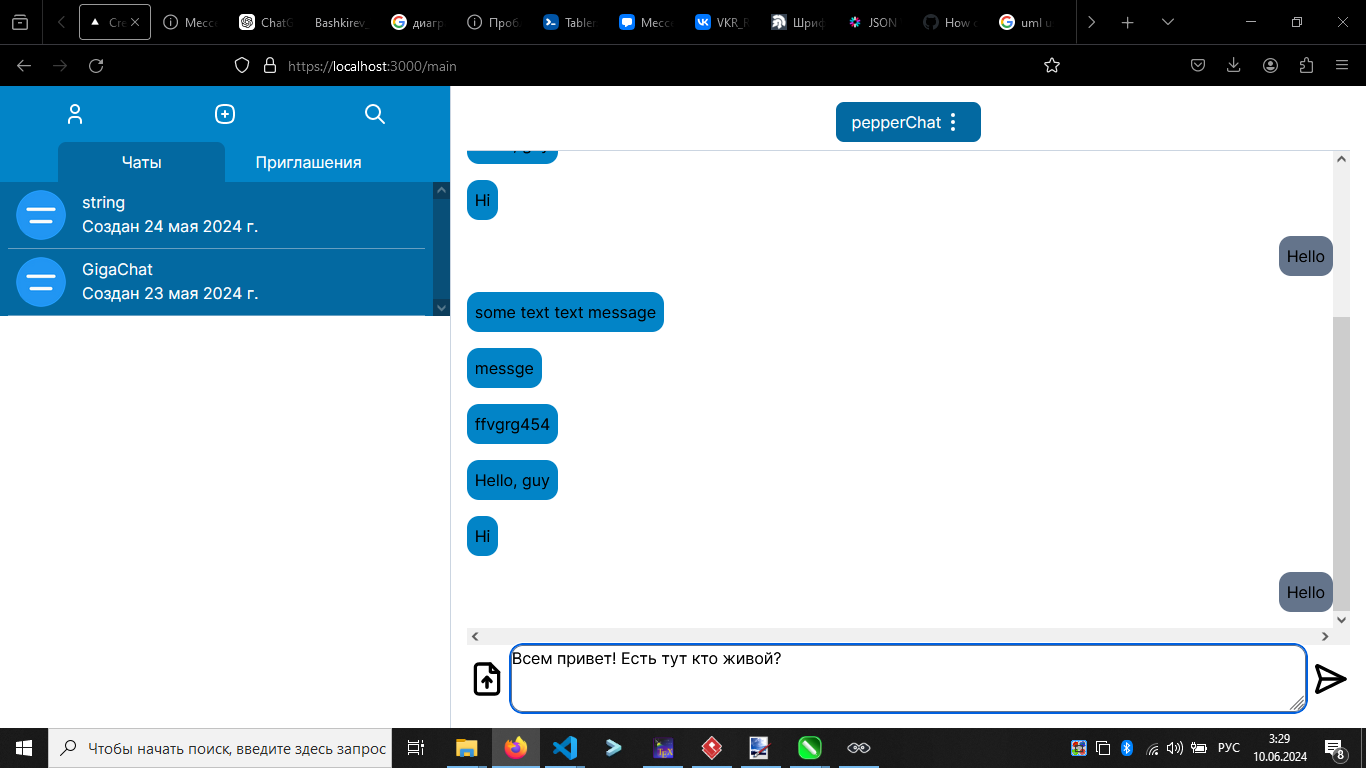
\includegraphics[width=1\linewidth]{newmessage_test1}}
	\caption{Вввод и отправка нового сообщения}
	\label{newmessage_test1:image}
\end{figure}

\begin{figure}[H]
	\center{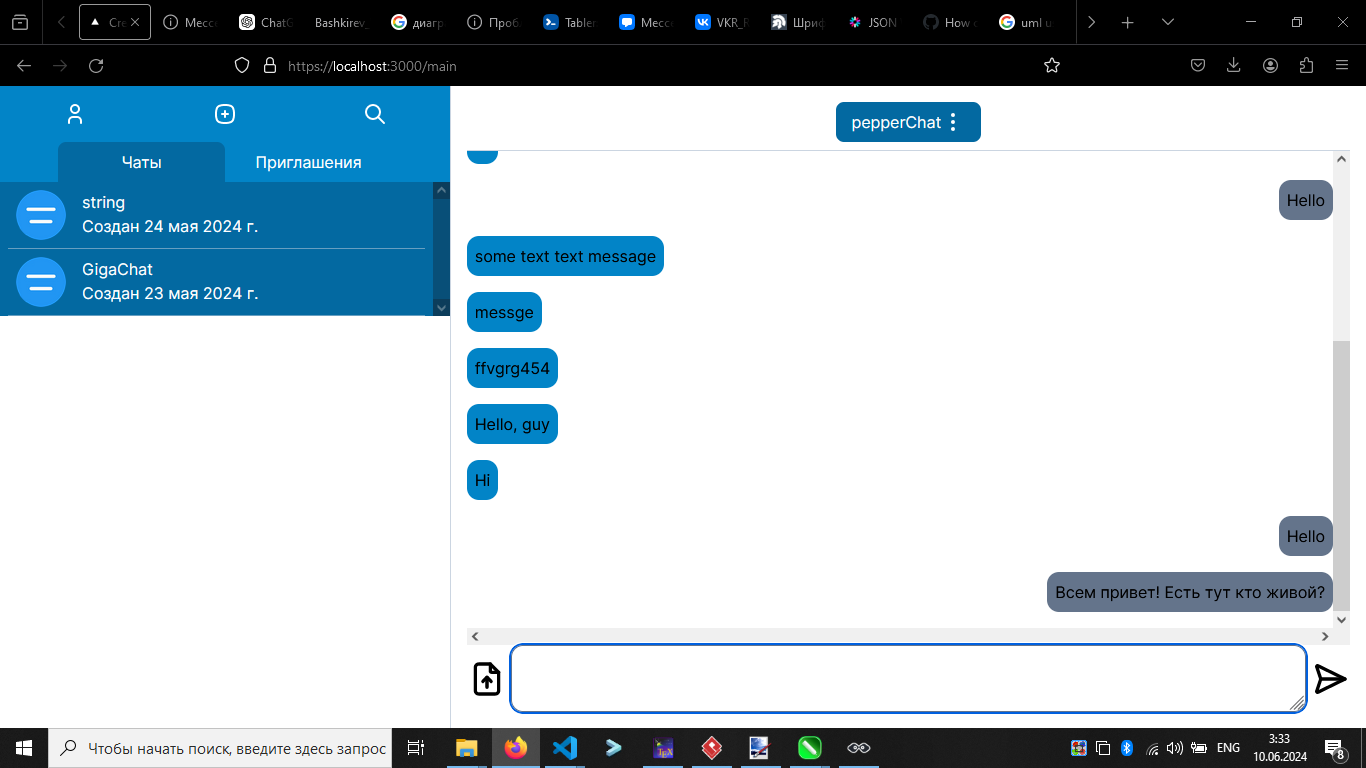
\includegraphics[width=1\linewidth]{newmessage_test2}}
	\caption{Результат отправки сообщения}
	\label{newmessage_test2:image}
\end{figure}

Произведем тестирование функционала входа в приложение. Для этого на странице входа в соответствующие поля необходимо ввести логин и пароль и нажать кнопку "<Войти">. Результаты тестирования представлены на рисунках.

\begin{figure}[H]
	\center{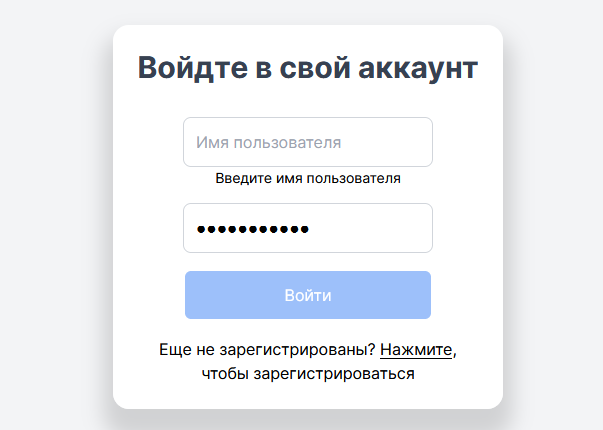
\includegraphics[width=1\linewidth]{signin_test1}}
	\caption{Попытка входа с неверными данными}
	\label{signin_test1:image}
\end{figure}

\begin{figure}[H]
	\center{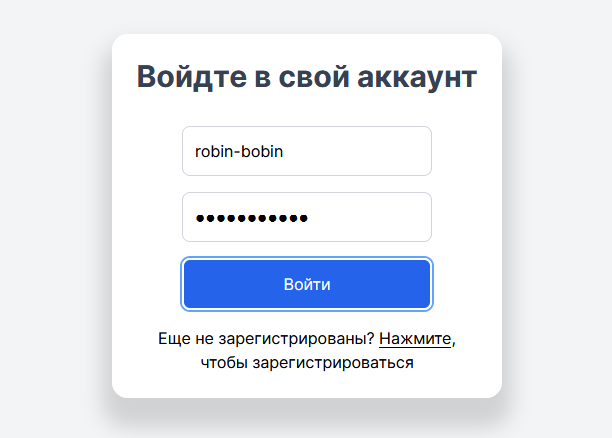
\includegraphics[width=1\linewidth]{signin_test2}}
	\caption{Ввод данных пользователя}
	\label{signin_test2:image}
\end{figure}

\begin{figure}[H]
	\center{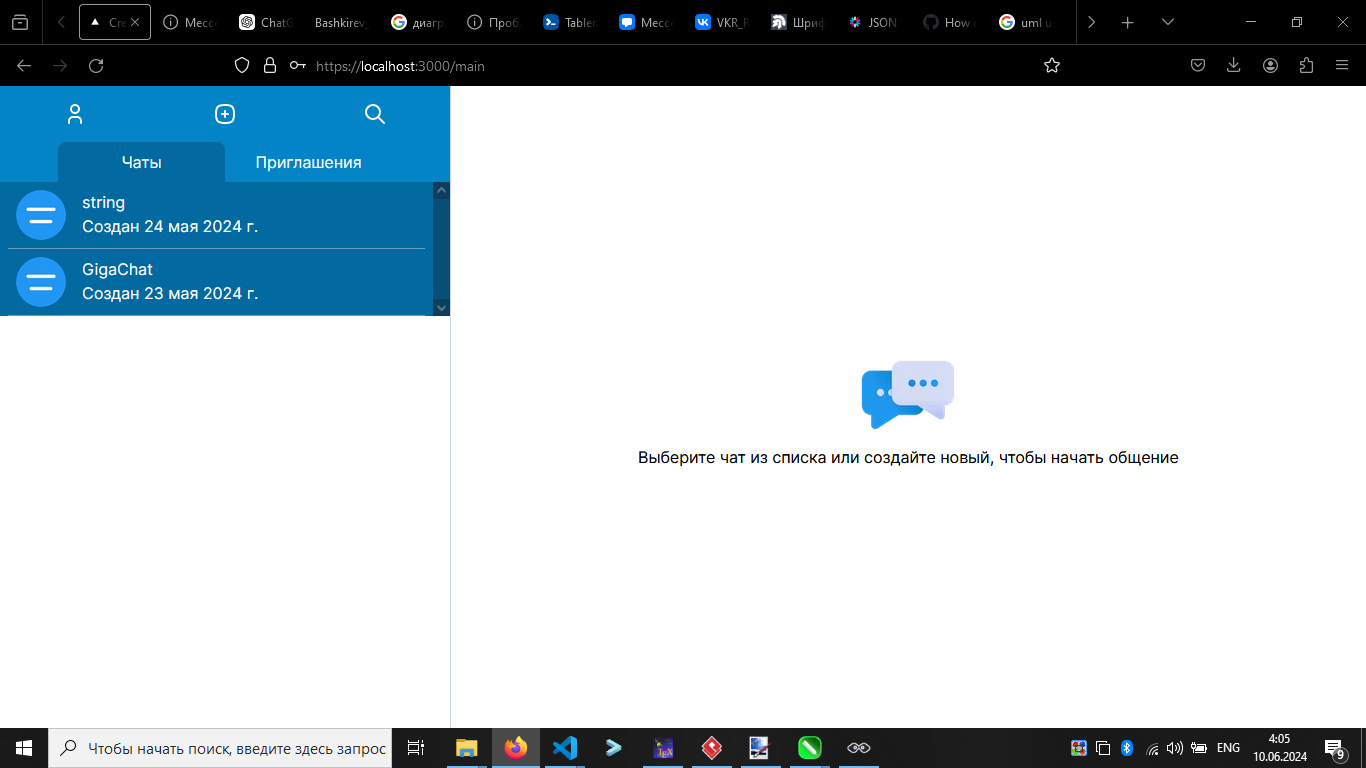
\includegraphics[width=1\linewidth]{signin_test3}}
	\caption{Главная страница после входа в приложение}
	\label{signin_test3:image}
\end{figure}